\documentclass{standalone}
\usepackage{tikz}
\usetikzlibrary{patterns, positioning}
\usetikzlibrary{shapes.misc}
\usepackage[outline]{contour}
\contourlength{1.5pt} 
\usepackage[sfdefault]{ClearSans} %% option 'sfdefault' activates Clear Sans as the default text font
\usepackage[T1]{fontenc}

\begin{document}
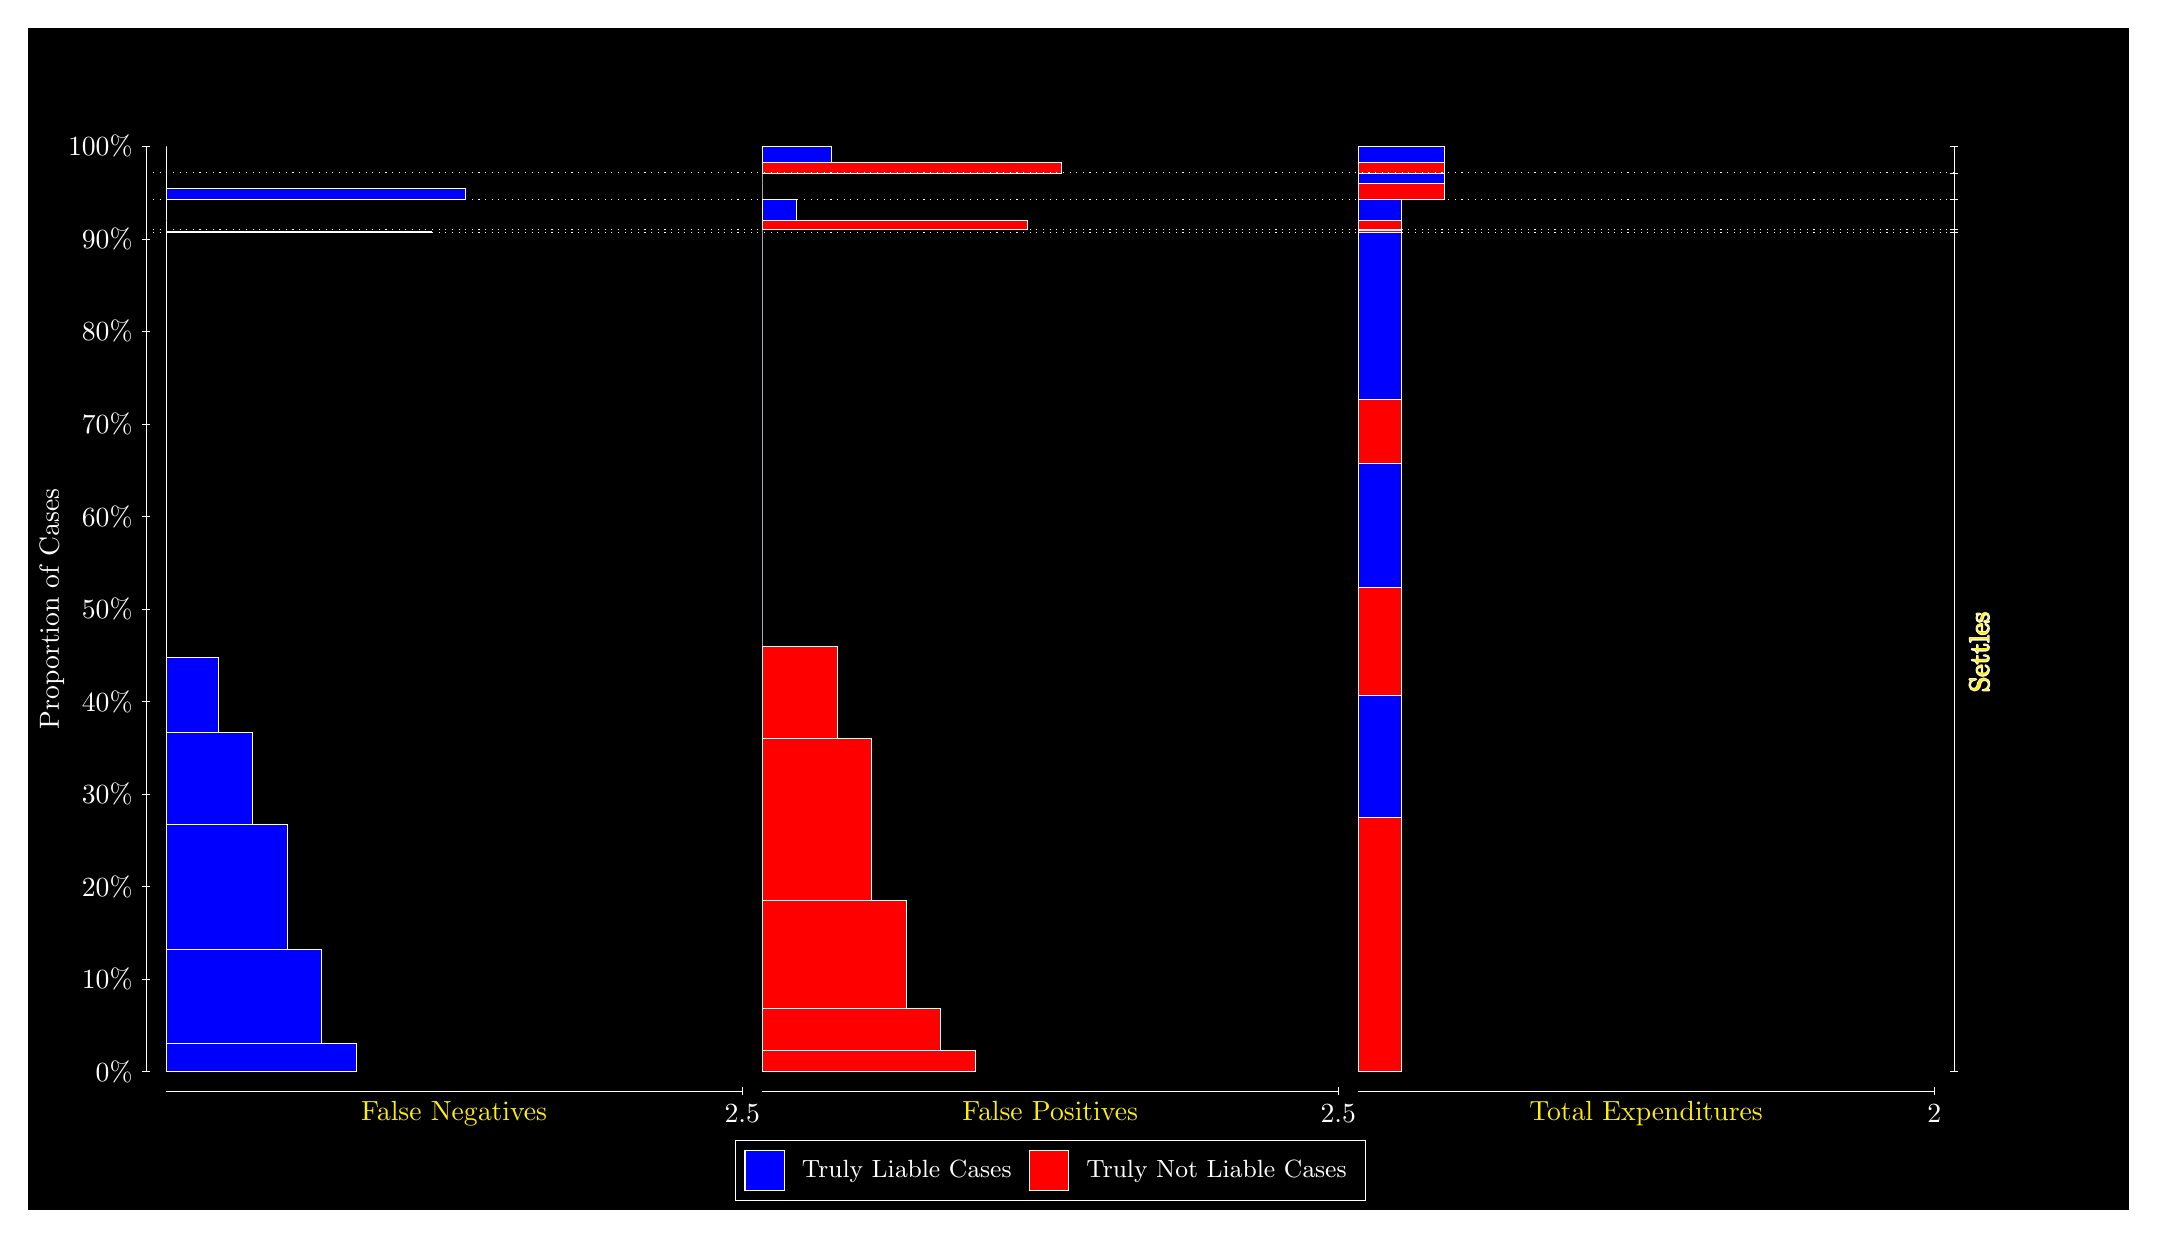
\begin{tikzpicture}
\draw[fill=black] (0,0) rectangle (26.667,15);
\draw[white, very thin] (1.5,1.75) -- (1.5,13.5);
\node[rotate=90, text=white, anchor=center] at (0.3, 7.625) {Proportion of Cases};
\draw[white, very thin] (1.45,1.75) -- (1.55,1.75);
\node[text=white, anchor=east] at (1.45, 1.75) {0\%};
\draw[white, very thin] (1.45,2.925) -- (1.55,2.925);
\node[text=white, anchor=east] at (1.45, 2.925) {10\%};
\draw[white, very thin] (1.45,4.1) -- (1.55,4.1);
\node[text=white, anchor=east] at (1.45, 4.1) {20\%};
\draw[white, very thin] (1.45,5.275) -- (1.55,5.275);
\node[text=white, anchor=east] at (1.45, 5.275) {30\%};
\draw[white, very thin] (1.45,6.45) -- (1.55,6.45);
\node[text=white, anchor=east] at (1.45, 6.45) {40\%};
\draw[white, very thin] (1.45,7.625) -- (1.55,7.625);
\node[text=white, anchor=east] at (1.45, 7.625) {50\%};
\draw[white, very thin] (1.45,8.8) -- (1.55,8.8);
\node[text=white, anchor=east] at (1.45, 8.8) {60\%};
\draw[white, very thin] (1.45,9.975) -- (1.55,9.975);
\node[text=white, anchor=east] at (1.45, 9.975) {70\%};
\draw[white, very thin] (1.45,11.15) -- (1.55,11.15);
\node[text=white, anchor=east] at (1.45, 11.15) {80\%};
\draw[white, very thin] (1.45,12.325) -- (1.55,12.325);
\node[text=white, anchor=east] at (1.45, 12.325) {90\%};
\draw[white, very thin] (1.45,13.5) -- (1.55,13.5);
\node[text=white, anchor=east] at (1.45, 13.5) {100\%};

\draw[white, very thin] (24.457,1.75) -- (24.457,13.5);
\draw[white, very thin] (24.407,1.75) -- (24.507,1.75);
\node[anchor=west] at (24.407, 1.75) {};
\draw[white, very thin] (24.407,12.405) -- (24.507,12.405);
\node[anchor=west] at (24.407, 12.405) {};
\draw[white, very thin] (24.407,12.445) -- (24.507,12.445);
\node[anchor=west] at (24.407, 12.445) {};
\draw[white, very thin] (24.407,12.829) -- (24.507,12.829);
\node[anchor=west] at (24.407, 12.829) {};
\draw[white, very thin] (24.407,13.164) -- (24.507,13.164);
\node[anchor=west] at (24.407, 13.164) {};
\draw[white, very thin] (24.407,13.5) -- (24.507,13.5);
\node[anchor=west] at (24.407, 13.5) {};

\draw[white, very thin, fill=blue] (1.75,1.75) rectangle (4.1652,2.1138);
\draw[white, very thin, fill=blue] (1.75,2.1138) rectangle (3.7261,3.3025);
\draw[white, very thin, fill=blue] (1.75,3.3025) rectangle (3.287,4.8865);
\draw[white, very thin, fill=blue] (1.75,4.8865) rectangle (2.8478,6.0621);
\draw[white, very thin, fill=blue] (1.75,6.0621) rectangle (2.4087,7.0084);
\draw[white, very thin, fill=red] (1.75,7.0084) rectangle (1.75,12.405);
\draw[white, very thin, fill=blue] (1.75,12.405) rectangle (5.1167,12.418);
\draw[white, very thin, fill=red] (1.75,12.418) rectangle (1.75,12.445);
\draw[white, very thin, fill=red] (1.75,12.445) rectangle (1.75,12.561);
\draw[white, very thin, fill=blue] (1.75,12.561) rectangle (1.75,12.829);
\draw[white, very thin, fill=blue] (1.75,12.829) rectangle (5.5558,12.965);
\draw[white, very thin, fill=red] (1.75,12.965) rectangle (1.75,13.164);
\draw[white, very thin, fill=red] (1.75,13.164) rectangle (1.75,13.299);
\draw[white, very thin, fill=blue] (1.75,13.299) rectangle (1.75,13.5);
\draw[white, very thin, fill=red] (9.3189,1.75) rectangle (12.027,2.0204);
\draw[white, very thin, fill=red] (9.3189,2.0204) rectangle (11.588,2.5549);
\draw[white, very thin, fill=red] (9.3189,2.5549) rectangle (11.149,3.919);
\draw[white, very thin, fill=red] (9.3189,3.919) rectangle (10.709,5.9857);
\draw[white, very thin, fill=red] (9.3189,5.9857) rectangle (10.27,7.1467);
\draw[white, very thin, fill=blue] (9.3189,7.1467) rectangle (9.3189,12.405);
\draw[white, very thin, fill=red] (9.3189,12.405) rectangle (9.3189,12.432);
\draw[white, very thin, fill=blue] (9.3189,12.432) rectangle (9.3189,12.445);
\draw[white, very thin, fill=red] (9.3189,12.445) rectangle (12.686,12.561);
\draw[white, very thin, fill=blue] (9.3189,12.561) rectangle (9.758,12.829);
\draw[white, very thin, fill=red] (9.3189,12.829) rectangle (9.3189,13.028);
\draw[white, very thin, fill=blue] (9.3189,13.028) rectangle (9.3189,13.164);
\draw[white, very thin, fill=red] (9.3189,13.164) rectangle (13.125,13.299);
\draw[white, very thin, fill=blue] (9.3189,13.299) rectangle (10.197,13.5);
\draw[white, very thin, fill=red] (16.888,1.75) rectangle (17.437,4.9778);
\draw[white, very thin, fill=blue] (16.888,4.9778) rectangle (17.437,6.5303);
\draw[white, very thin, fill=red] (16.888,6.5303) rectangle (17.437,7.8944);
\draw[white, very thin, fill=blue] (16.888,7.8944) rectangle (17.437,9.4784);
\draw[white, very thin, fill=red] (16.888,9.4784) rectangle (17.437,10.283);
\draw[white, very thin, fill=blue] (16.888,10.283) rectangle (17.437,12.405);
\draw[white, very thin, fill=red] (16.888,12.405) rectangle (17.437,12.432);
\draw[white, very thin, fill=blue] (16.888,12.432) rectangle (17.437,12.445);
\draw[white, very thin, fill=red] (16.888,12.445) rectangle (17.437,12.561);
\draw[white, very thin, fill=blue] (16.888,12.561) rectangle (17.437,12.829);
\draw[white, very thin, fill=red] (16.888,12.829) rectangle (17.986,13.028);
\draw[white, very thin, fill=blue] (16.888,13.028) rectangle (17.986,13.164);
\draw[white, very thin, fill=red] (16.888,13.164) rectangle (17.986,13.299);
\draw[white, very thin, fill=blue] (16.888,13.299) rectangle (17.986,13.5);
\draw[white, dotted] (1.5,12.405) -- (24.457,12.405);
\draw[white, dotted] (1.5,12.445) -- (24.457,12.445);
\draw[white, dotted] (1.5,12.829) -- (24.457,12.829);
\draw[white, dotted] (1.5,13.164) -- (24.457,13.164);
\draw[white, very thin] (1.75,1.5) -- (9.0689,1.5);
\node[text=yellow, anchor=north] at (5.4094, 1.5) {False Negatives};
\draw[white, very thin] (9.0689,1.45) -- (9.0689,1.55);
\node[text=white, anchor=north] at (9.0689, 1.45) {2.5};

\draw[white, very thin] (9.3189,1.5) -- (16.638,1.5);
\node[text=yellow, anchor=north] at (12.978, 1.5) {False Positives};
\draw[white, very thin] (16.638,1.45) -- (16.638,1.55);
\node[text=white, anchor=north] at (16.638, 1.45) {2.5};

\draw[white, very thin] (16.888,1.5) -- (24.207,1.5);
\node[text=yellow, anchor=north] at (20.547, 1.5) {Total Expenditures};
\draw[white, very thin] (24.207,1.45) -- (24.207,1.55);
\node[text=white, anchor=north] at (24.207, 1.45) {2};

\node[text=yellow, centered, rotate=90] at (24.777, 7.0776) {\contour{white}{Settles}};





\draw (12.978300999999998,1.5) node[draw=none] (baseCoordinate) {};
\begin{scope}[align=center]
        \matrix[scale=0.5, draw=white, below=0.5cm of baseCoordinate, nodes={draw}, column sep=0.1cm]{
            \node[rectangle, draw, minimum width=0.5cm, minimum height=0.5cm, fill=blue] {}; &
            \node[draw=none, font=\small, text=white] (B) {Truly Liable Cases}; &
            \node[rectangle, draw, minimum width=0.5cm, minimum height=0.5cm, fill=red] {}; &
            \node[draw=none, font=\small, text=white] (B) {Truly Not Liable Cases}; \\
            };
\end{scope}

\end{tikzpicture}
\end{document}